\subsection{Functional Architecture}

\begin{frame}
\frametitle{Functional Architecture}
The functional architecture is initially developed during the research phase
and refined as development matures to production.

\begin{itemize}
    \item The main components of a system are identified
    \item Specific algorithms which realize the components are developed
    \item High-level interfaces between components are created
\end{itemize}

\begin{block}{}
The functional architecture for an autonomous driving vehicle has evolved
over the past decade and is converging towards an industry standard.
\end{block}
\end{frame}

\begin{frame}
\frametitle{Sense - Plan - Act}
\framesubtitle{Common Autonomous Vehicle Functional Architecture}
The \emph{Sense - Plan - Act} architecture is still predominant in modern autonomous
vehicle architectures.

\vspace{1cm}

\begin{center}
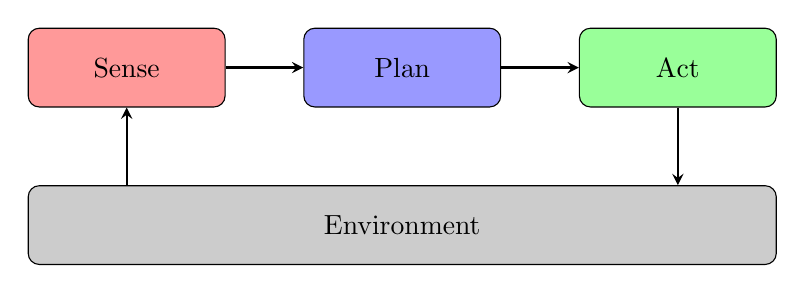
\begin{tikzpicture}[node distance=3.5cm]
    \node (sense)[rectangle,rounded corners,minimum width=2.5cm,minimum height=1cm,text centered,draw=black,fill=red!40]{Sense};
    \node (plan)[right of=sense,rectangle,rounded corners,minimum width=2.5cm,minimum height=1cm,text centered,draw=black,fill=blue!40]{Plan};
    \node (act)[right of=plan,rectangle,rounded corners,minimum width=2.5cm,minimum height=1cm,text centered,draw=black,fill=green!40]{Act};
    \node (environment)[below of=plan,yshift=1.5cm,rectangle,rounded corners,minimum width=9.5cm,minimum height=1cm,text centered,draw=black,fill=gray!40]{Environment};
    \draw [thick,->,>=stealth] (sense) -- (plan);
    \draw [thick,->,>=stealth] (plan) -- (act);
    \draw [thick,->,>=stealth] (act) -- ([xshift=3.5cm]environment.north);
    \draw [thick,<-,>=stealth] (sense) -- ([xshift=-3.5cm]environment.north);
    \end{tikzpicture}
\end{center}
\end{frame}

\begin{frame}
\frametitle{Sense - Plan - Act}
\framesubtitle{Common Autonomous Vehicle Functional Architecture}
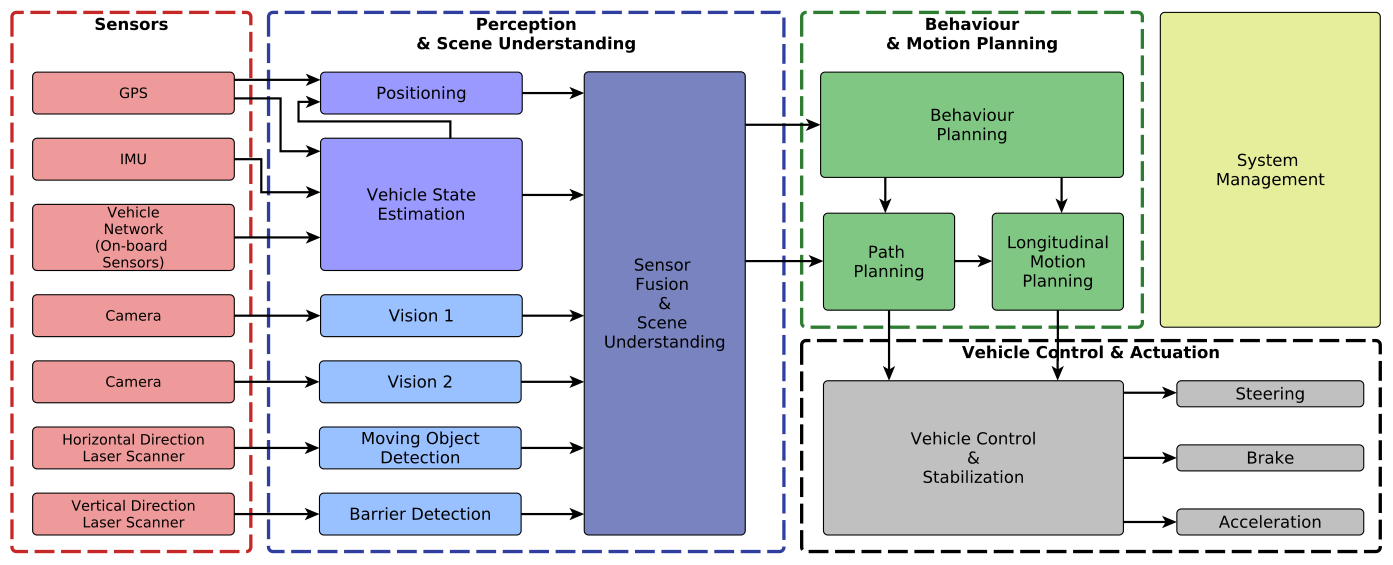
\includegraphics[width=\textwidth]{images/tas_2016_fig4_av_functional_architecture.png}
\tiny{Architecture image from \cite{Tas2016-sd} based on the vehicle that won the
Korean Autonomous Vehicle Competition \cite{Jo2014-na}}.
\end{frame}

\begin{frame}
\frametitle{Sensors}
Autonomous vehicles use a combination of cameras, radar and lidar sensors to
sense and perceive the environment. \\
\vspace{0.5cm}
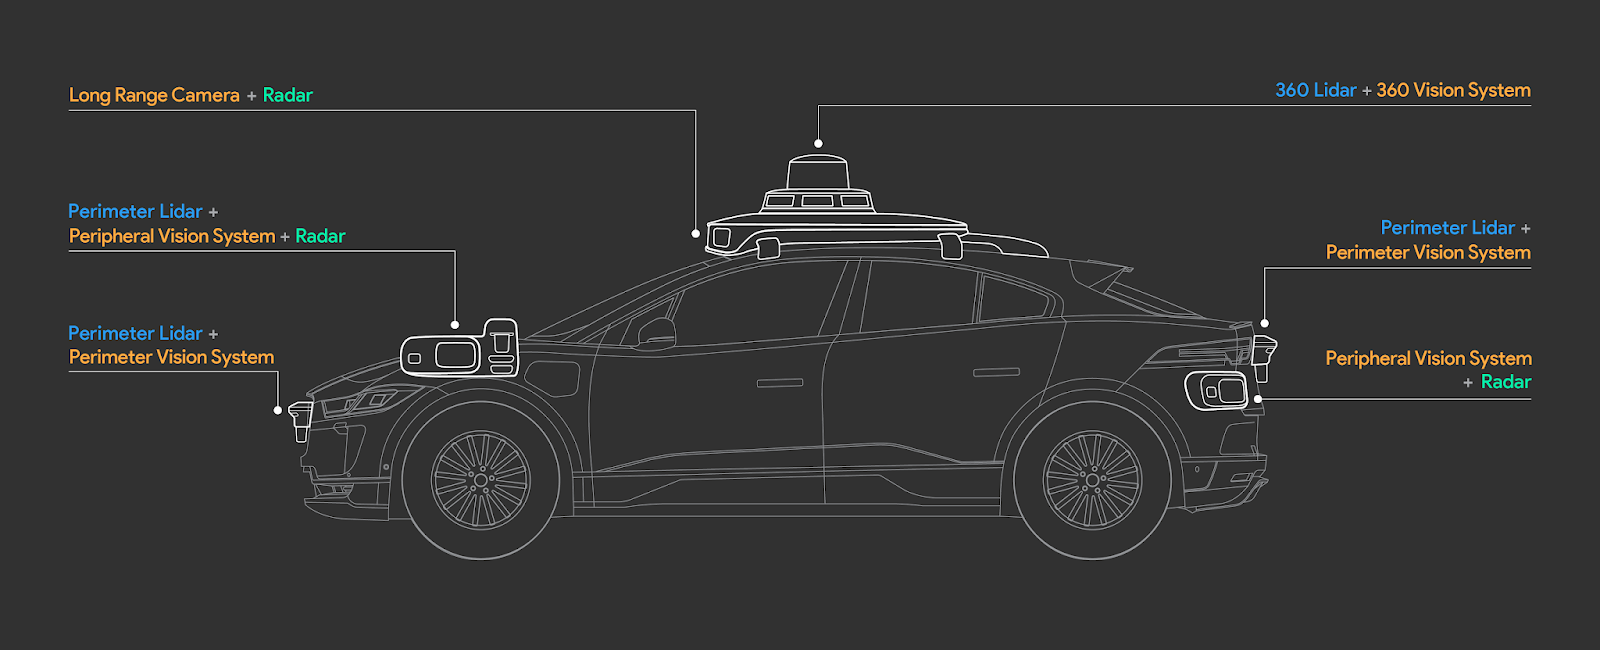
\includegraphics[width=\textwidth]{images/waymo_sensors.png}
\footnotesize{Waymo sensor suite\footnotemark[1]}
\footnotetext[1]{\tiny{\url{https://blog.waymo.com/2020/03/introducing-5th-generation-waymo-driver.html}}}
\end{frame}

\begin{frame}
\frametitle{Sensors}
\framesubtitle{Camera}
\begin{columns}[T]
    \begin{column}{.5\textwidth}
        \centering
        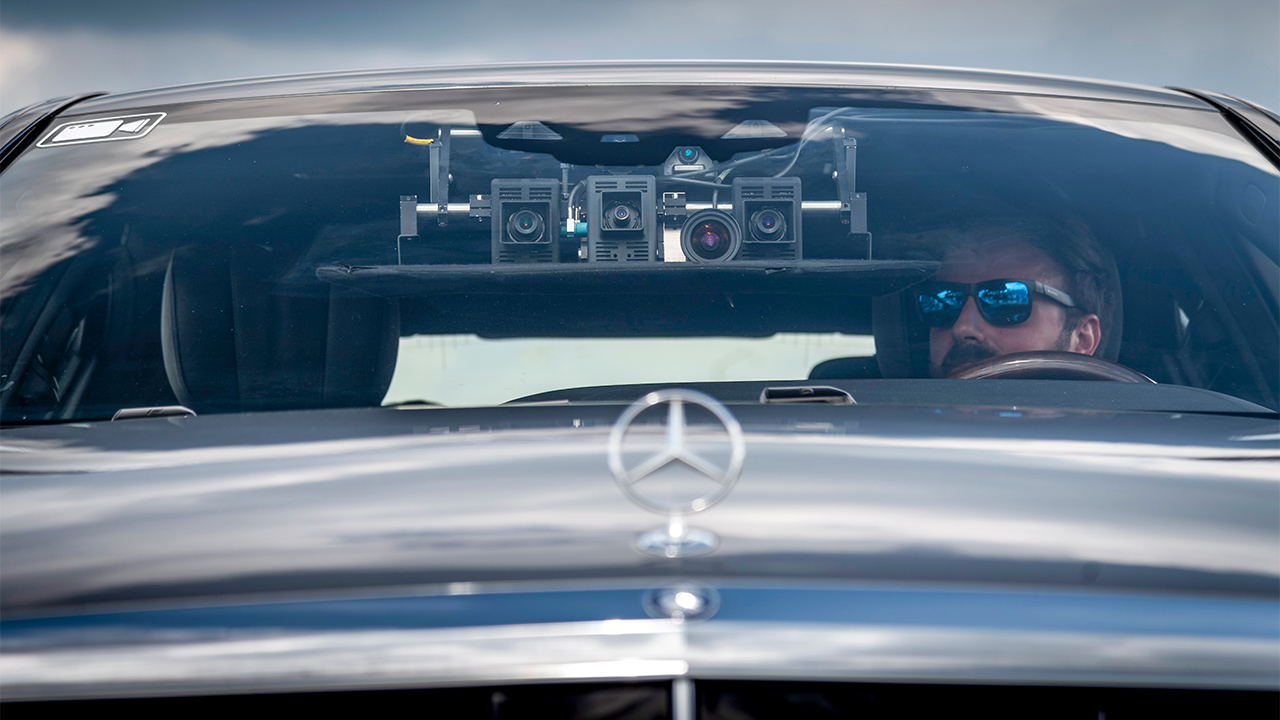
\includegraphics[height=2.0cm]{images/daimler_cameras.jpg}\\
        \tiny{Source: Daimler\footnotemark[1]}
    \end{column}
    \begin{column}{.5\textwidth}
        \centering
        \href{https://www.youtube.com/watch?v=rACZACXgreQ}{
        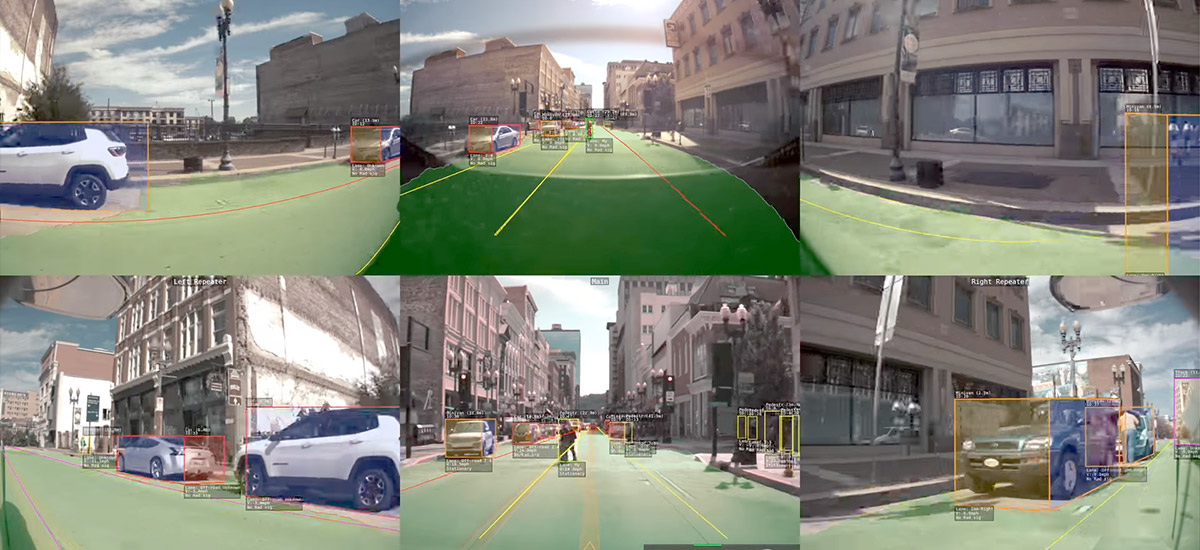
\includegraphics[height=2.0cm]{images/tesla_autopilot_cameras.jpg}}\\
        \tiny{Tesla camera system, Source: YouTube (greentheonly)\footnotemark[2]}
    \end{column}
\end{columns}

\vspace{0.2cm}

\footnotesize
Vision sensors are the basis for an autonomous driving system, providing
important perception input for many different purposes.

\begin{columns}[T]
    \begin{column}{0.45\textwidth}
        \footnotesize
        Capabilities:
        \begin{itemize}
            \item Dynamic object detection
            \item Static object detection
            \item Lane and road detection
            \item Classification
            \item Traffic sign/light detection
        \end{itemize}
    \end{column}
    \begin{column}{0.55\textwidth}
        \footnotesize
        Important properties:
        \begin{itemize}
            \item High dynamic range
            \item $360\deg$ field of view
            \item Global shutter
            \item Low cost
            \item No distance or velocity measurements
        \end{itemize}
    \end{column}
\end{columns}

\footnotetext[1]{\tiny{\url{https://www.daimler.com/magazine/technology-innovation/automation-daimler-immendingen-camera-radar-lidar.html}}}
\footnotetext[2]{\tiny{\url{https://www.youtube.com/watch?v=rACZACXgreQ}}}
\end{frame}

\begin{frame}
\frametitle{Sensors}
\framesubtitle{Radar}
\begin{columns}[b]
    \begin{column}{.5\textwidth}
        \centering
        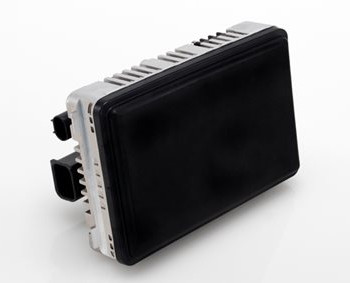
\includegraphics[height=2.0cm]{images/continental_radar.jpg}\\
        \vspace{0.2cm}
        \tiny{Source: Continental\footnotemark[1]}
    \end{column}
    \begin{column}{.5\textwidth}
        \centering
        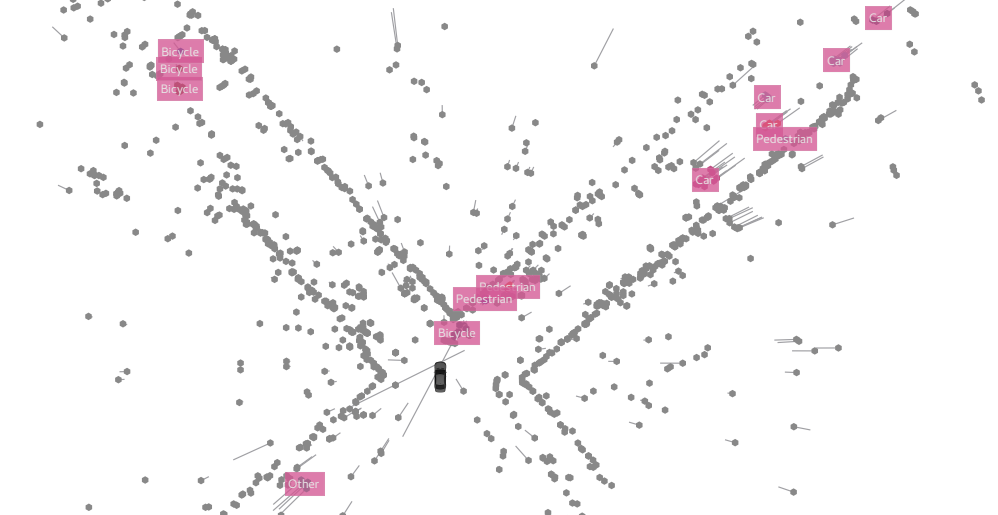
\includegraphics[height=2.5cm]{images/daimler_radar_dataset.png}\\
        \tiny{Source: Daimler, RadarScene dataset\footnotemark[2]}
    \end{column}
\end{columns}

\vspace{0.2cm}

\footnotesize
Radar has been the workhorse of ADAS for over two decades, being the main
sensor for ACC and continues its importance in autonomous driving systems.

\begin{columns}[T]
    \begin{column}{0.4\textwidth}
        \footnotesize
        Capabilities:
        \begin{itemize}
            \item Dynamic object detection
            \item Static object detection
            \item Road boundary detection
        \end{itemize}
    \end{column}
    \begin{column}{0.6\textwidth}
        \footnotesize
        Important properties:
        \begin{itemize}
            \item Robust in weather, e.g. rain, fog, etc.
            \item Direct measurement of speed
            \item Reasonable cost
            \item Low resolution, poor vertical separation
        \end{itemize}
    \end{column}
\end{columns}
\footnotetext[1]{\tiny{\url{https://www.continental-automotive.com/en-gl/Passenger-Cars/Autonomous-Mobility/Enablers/Radars/Long-Range-Radar/ARS540}}}
\footnotetext[2]{\tiny{\url{https://radar-scenes.com/}}}
\end{frame}

\begin{frame}
\frametitle{Sensors}
\framesubtitle{Lidar}
\begin{columns}[T]
    \begin{column}{.5\textwidth}
        \centering
        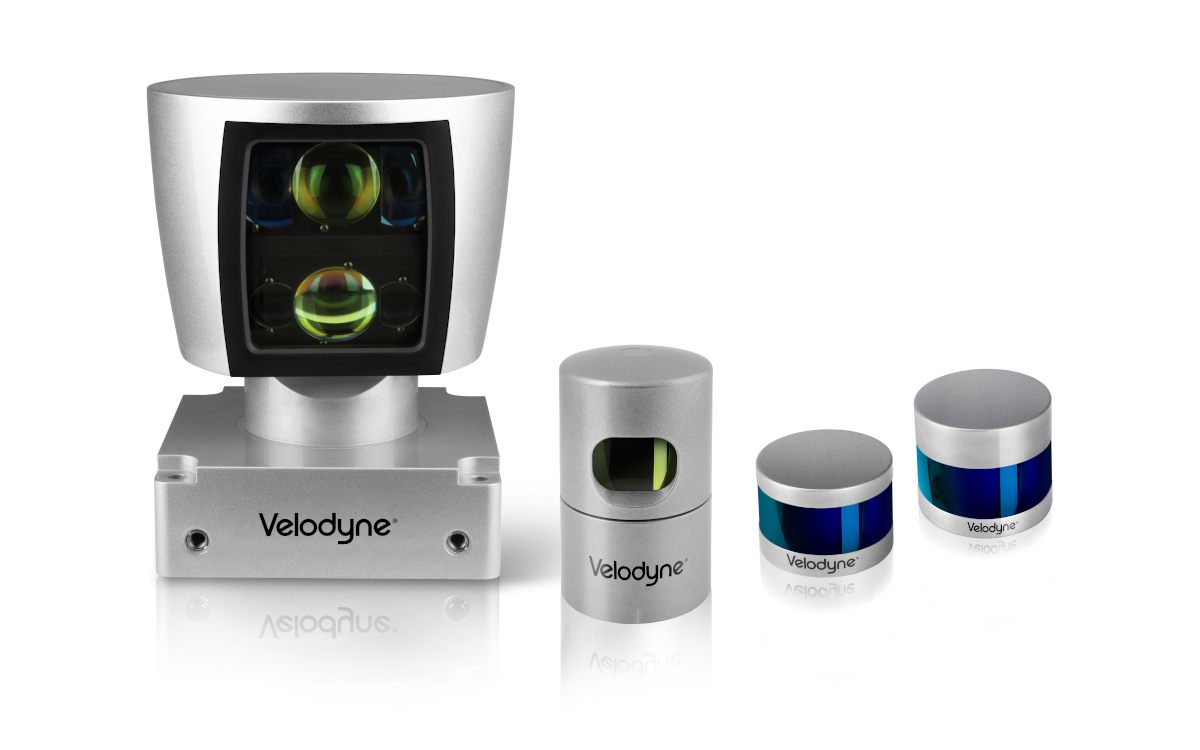
\includegraphics[height=2.5cm]{images/velodyne_lidars.png}\\
        \tiny{Source: Velodyne\footnotemark[1]}
    \end{column}
    \begin{column}{.5\textwidth}
        \centering
        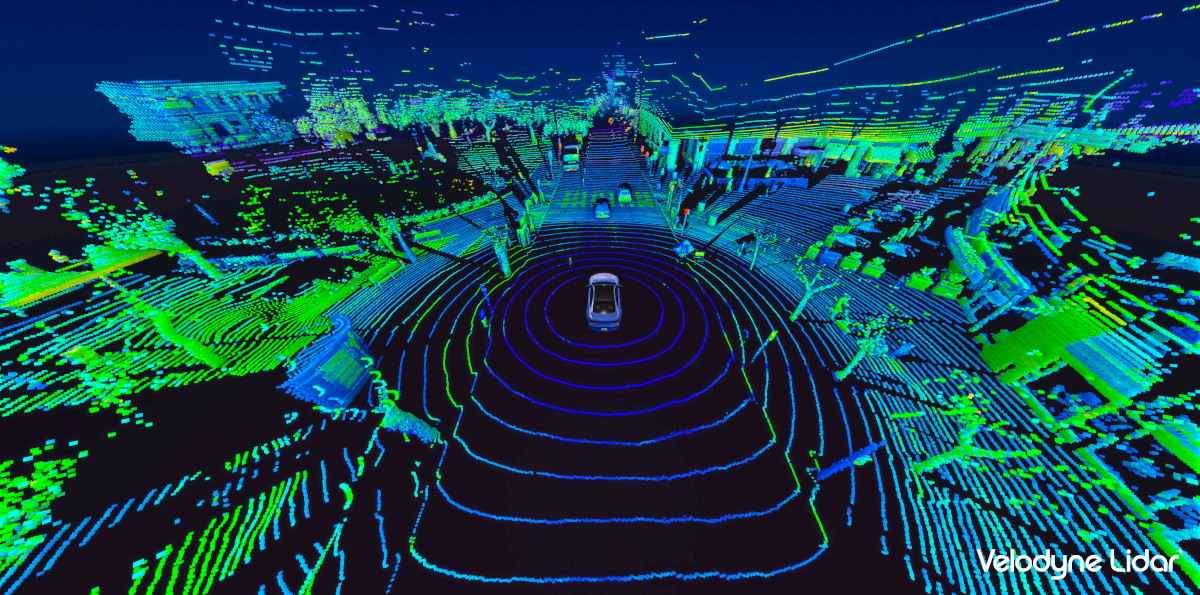
\includegraphics[height=2.5cm]{images/velodyne_pointcloud.jpg}\\
        \tiny{Source: Velodyne\footnotemark[1]}
    \end{column}
\end{columns}

\vspace{0.2cm}

\footnotesize
Only very recently has lidar been introduced in production vehicles, but it has
been a core sensor of autonomous driving research since the DARPA challenges.

\begin{columns}[T]
    \begin{column}{0.4\textwidth}
        \footnotesize
        Capabilities:
        \begin{itemize}
            \item Dynamic and static object detection
            \item Road boundary and curb detection
            \item Lane detection
        \end{itemize}
    \end{column}
    \begin{column}{0.6\textwidth}
        \footnotesize
        Important properties:
        \begin{itemize}
            \item High resolution
            \item Large field of view
            \item Measure intensity
            \item Poor weather robustness
            \item No velocity measurement
        \end{itemize}
    \end{column}
\end{columns}
\footnotetext[1]{\tiny{\url{https://velodynelidar.com/media-kit/}}}
\end{frame}

\begin{frame}
\frametitle{Perception}
\framesubtitle{Object Detection and Tracking}

\end{frame}

\begin{frame}S
\frametitle{Perception}
\framesubtitle{Occupancy Grids}

\end{frame}

\begin{frame}
\frametitle{Perception}
\framesubtitle{Sensor Data Fusion}

\end{frame}

\begin{frame}
\frametitle{Localization}

\end{frame}

\begin{frame}
\frametitle{Prediction}

\end{frame}

\begin{frame}
\frametitle{Motion Planning}

\end{frame}

\begin{frame}
\frametitle{Vehicle Control}

\end{frame}

\begin{frame}
\frametitle{Machine Learning in Autonomous Driving}

\end{frame}